\documentclass[pdf,xcolor={dvipsnames}]{beamer}
\usepackage{xcolor,soul}
% \renewcommand<>{\hl}[1]{\only#2{\beameroriginal{\hl}}{#1}}

\mode<presentation>{\usetheme{default}}
\title{Improving an Exact Solution to the \newline ($l$,$d$) Planted Motif Problem}
\author{Maria Clara Isabel Sia}

\definecolor{green}{HTML}{4CBB17}
% \AtBeginSection[]{
% 	\begin{frame}{}\tableofcontents[currentsection]\end{frame}
% }

\begin{document}

\begin{frame}
\titlepage
\end{frame}

\section{Introduction}
	\begin{frame}{Introduction}{DNA motif finding}
		\begin{itemize}
			\item motifs: repeated sub-sequences in DNA that have some biological significance\newline
			\item DNA motif finding: search for motifs over a set of DNA sequences, allowing for mismatches due to mutation\newline
			\item known as a difficult problem in computational biology and CS (proven NP-complete)\newline
		\end{itemize}
		\end{frame}

	\subsection{The ($l$,$d$) planted motif problem}
	\begin{frame}{Introduction}{The ($l$,$d$) planted motif problem}
		% Given a set $\mathcal{S} = \{S_{1},...S_{n}\}$ of $n$ DNA sequences of length $L$,
		% \newline \hspace*{12pt} find $M$, the set of sub-sequences (motifs) of length $l < L$
		% \newline \hspace*{12pt} which occur with at most $d$ mismatches in each sequence in $\mathcal{S}$.
		% \newline
		\centering
		\emph{Find a motif of length $l$=8 across 5 DNA sequences,}\\
		\emph{each containing the motif with at most $d$=2 mismatches.}\\
		\ \\
		% ($l$, $d$) = (8, 2)\\
		\footnotesize
		% \ \\
		$S_1$\ \ \  \texttt{at{\color{blue}c{ac}tcgtt}ctcctctaatgtgtaaagacgtactaccgacctta}\\
		$S_2$\ \ \  \texttt{acgccgaccggtc{\color{blue}c{g}atc{c}tt}gtatagctcctaacgggcatcagc}\\
		$S_3$\ \ \  \texttt{tcctgactgcatcgcgatctcggtagtttcctgt{\color{blue}{t}catc{a}tt}ttt}\\
		$S_4$\ \ \  \texttt{ggccctca{\color{blue}{g}catcgt{g}}cgtcctgctaacacattcccatgcagctt}\\
		$S_5$\ \ \  \texttt{tgaaaagaatttacggtaaaggatccacatc{\color{blue}c{a}atcgt{g}}tgaaag}\\ 
		\ \\
		\emph{Planted motif: }\texttt{\color{blue}ccatcgtt}\\

		Given: set of DNA sequences $\mathcal{S} = \{S_{1},...S_{n}\}$, motif length $l$, allowable mismatches $d$
		
		\end{frame}

	\subsection{$l$-mers, Hamming distances, and $d$-neighborhoods}
	\begin{frame}{Introduction}{$l$-mers, Hamming distances, and $d$-neighborhoods}
		\begin{itemize}
		\setbeamercovered{transparent=25}
		\item<1,2>
			\alt<2>{{\usebeamercolor[fg]{frametitle} $l$-mer}}
													{$l$-mer}
			\only<2>{ \newline- sequence of length $l$\newline
				\newline
				{\footnotesize
				\hspace*{0.05\textwidth}$l$ = 8,\newline
				\hspace*{0.05\textwidth}$S$ = \texttt{acgccgattacatc{\color{red}cgatcctt}gtatagctcctaacgggcatcac}\newline
				{\color{blue}\hspace*{0.35\textwidth} $\hookrightarrow$ $15^{th}$ $l$-mer in $S$\newline}
				% \newline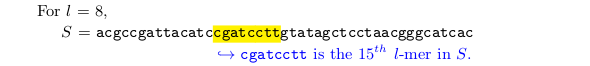
\includegraphics[width=11.0cm]{img/concepts_lmer}
				}
			}
		\item<1,3>
			\alt<3>{{\usebeamercolor[fg]{frametitle} Hamming distance $dH(x_1, x_2)$}}
													{Hamming distance $dH(x_1, x_2)$}
			\only<3>{ \newline- number of mismatches between $l$-mers $x_1$ and $x_2$\newline
				\newline
				{\footnotesize
				\hspace*{0.15\textwidth} $x_1$ = \texttt{c{\color{red}g}atc{\color{red}c}tt}\newline
				\hspace*{0.15\textwidth} $x_2$ = \texttt{c{\color{red} c}atc{\color{red} g}tt}\newline
				{\color{blue} \hspace*{0.25\textwidth}
					$\hookrightarrow$ $2^{nd}$ and $6^{th}$ characters differ\newline
					\hspace*{0.27\textwidth} thus, $dH(x_1, x_2)$ = 2.\newline
					}
				}
				% \newline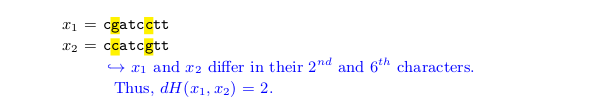
\includegraphics[width=11.0cm]{img/concepts_dH}		
			}
		\item<1,4>
			\alt<4>{{\usebeamercolor[fg]{frametitle} $d$-neighborhood $N(x,d)$ of $l$-mer $x$}} 
													{$d$-neighborhood $N(x,d)$ of $l$-mer $x$}
			\only<4>{ \newline- set of all $l$-mers having at most $d$ mismatches with $x$\newline
				\newline
				{\footnotesize 
					$N$(\texttt{ccatcgtt}, 2) = \{ \texttt{ccatcgtt}, \newline
					\texttt{
						\hspace*{0.1\textwidth}
						{\color{red}a}catcgtt,{\color{green}g}catcgtt,{\color{blue}t}catcgtt,%
						c{\color{red}a}atcgtt,c{\color{green}g}atcgtt,c{\color{blue}t}atcgtt,
					}	
					\hspace*{0.12\textwidth}...
					\hspace*{0.35\textwidth}{\color{blue} $\hookrightarrow$ 1 mismatch}\newline
					\texttt{
						\hspace*{0.1\textwidth}
						{\color{red}a}{\color{red}a}atcgtt,%
						{\color{red}a}{\color{green}g}atcgtt,%
						{\color{red}a}{\color{blue}t}atcgtt,%
						{\color{green}g}{\color{red}a}atcgtt,%
						{\color{green}g}{\color{green}g}atcgtt,%
						{\color{green}g}{\color{blue}t}atcgtt,
						\hspace*{0.1\textwidth}
						{\color{blue}t}{\color{red}a}atcgtt,%
						{\color{blue}t}{\color{green}g}atcgtt,%
						{\color{blue}t}{\color{blue}t}atcgtt,%
						{\color{red}a}c{\color{red}c}tcgtt,%
						{\color{red}a}c{\color{green}g}tcgtt,%
						{\color{red}a}c{\color{blue}t}tcgtt,					
				 	}
				 	\hspace*{0.12\textwidth}...
				 	\hspace*{0.35\textwidth}{\color{blue} $\hookrightarrow$ 2 mismatches}\newline
				 	\hspace*{0.12\textwidth}{\footnotesize\}}
			 	}
				% \newline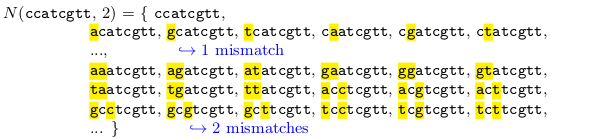
\includegraphics[width=10.5cm]{img/concepts_N(x,d)}	
				}
		\item<1,5>
			\alt<5>{{\usebeamercolor[fg]{frametitle} $d$-neighborhood $\mathcal{N}(S,d)$ of sequence $S$}}
													{$d$-neighborhood $\mathcal{N}(S,d)$ of sequence $S$}
			\only<5>{ \newline- set of all $d$-neighbors of all $l$-mers in $S$\newline\newline
			{\footnotesize
			\hspace*{0.08\textwidth}$S$ = \texttt{{\color{green}acgccgat}tacatc{\color{red}cgatcctt}gtatagctcctaacg{\color{blue}ggcatcac}}\newline
			% \hspace*{0.05\textwidth}
				$\mathcal{N}(S, 2)$ = 
					$N$(\texttt{\color{green}  acgccgat}, 2) $\cup ...\cup$
					$N$(\texttt{\color{red}cgatcctt}, 2) $\cup ...\cup$
					$N$(\texttt{\color{blue} ggcatcac}, 2)\newline
				\hspace*{0.05\textwidth} {\color{blue} $\hookrightarrow$ union of $d$-neighborhoods of $l$-mers in $S$}
			}
			% \newline\newline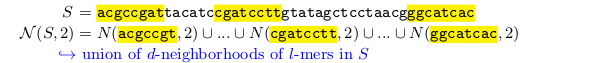
\includegraphics[width=11.0cm]{img/concepts_N(S,d)}		
		}
		\end{itemize}
		\end{frame}

\section{EMS-GT}
	\begin{frame}{EMS-GT}{Nabos, 2014}
		\begin{itemize}
		\item an exact motif search (EMS) algorithm based on the candidate generate-and-test (GT) principle\newline
		\item solves the ($l$,$d$) planted motif problem for any arbitrary instance with $l \leq 17$ \newline
		\item efficiently operates on a compact, bit-based representation of the motif search space
		\end{itemize}
		\end{frame}

	\subsection{Generate-and-test approach}
	\begin{frame}{EMS-GT}{Generate-and-test approach}
		% The EMS-GT algorithm proceeds in two main steps:\newline
		\only<1>{
			EMS-GT proceeds in two steps:\newline
			\begin{enumerate}
			\item % Generate candidate motifs\newline
			{\usebeamercolor[fg]{frametitle}Generate the set $C$ of candidate motifs}: find
			the common neighbors of the first $n'$ sequences $S_1,S_2,...,S_{n'}$.\newline\newline
			% as the intersection of the $d$-neighborhoods of the first $n'$ sequences $S_1,S_2,...,S_{n'}$.\newline\newline
			\hspace*{14pt} {$C = \mathcal{N}(S_1,d) \cap \mathcal{N}(S_2,d) \cap ... \cap \mathcal{N}(S_{n'},d) ),
			\ \ \ \ n' \leq n $\newline}

			% . Every $l$-mer in the resulting set $C$ is a candidate motif.\newline
			\item % Test candidates\newline
			{\usebeamercolor[fg]{frametitle}Test every candidate $c \in C$}: if a $d$-neighbor of $c$ appears in each of the remaining sequences $S_{n'+1},S_{n'+2},...S_n$, accept $c$ as a motif.
			\end{enumerate}
		}

		 \only<2>{
		 	\bigskip\bigskip
		 	($l$,$d$) = (8,2)\newline\newline\newline
		 	\footnotesize
			$S_1$\ \ \  \texttt{at{c{ac}tcgtt}ctcctctaatgtgtaaagacgtactaccgacctta}\newline\newline\newline
			$S_2$\ \ \  \texttt{acgccgaccggtc{c{g}atc{c}tt}gtatagctcctaacgggcatcagc}\newline\newline\newline
			$S_3$\ \ \  \texttt{tcctgactgcatcgcgatctcggtagtttcctgt{{t}catc{a}tt}ttt}\newline\newline\newline

			$S_4$\ \ \  \texttt{ggccctca{{g}catcgt{g}}cgtcctgctaacacattcccatgcagctt}\newline\newline\newline
			$S_5$\ \ \  \texttt{tgaaaagaatttacggtaaaggatccacatc{c{a}atcgt{g}}tgaaag}\newline\newline\newline
		% 	includegraphics[width=10.0]{ems-gt_demo}
		 }
		\end{frame}

	\subsection{Bit-based efficiency strategies}
	\begin{frame}{EMS-GT}{Bit-based efficiency strategies}
		\begin{itemize}
		\setbeamercovered{transparent=25}
		\item<1,2> \alt<2>{{\usebeamercolor[fg]{frametitle}$l$-mer enumeration scheme}}{$l$-mer enumeration scheme}
			\only<2>{
				\newline EMS-GT maps an $l$-mer to a $2l$-bit binary number by replacing each
			character with two bits (\texttt{a=00}, \texttt{c=01}, \texttt{g=10}, \texttt{t=11}).\newline\newline
			% This scheme enumerates $l$-mers in alphabetical order.
				{
				\scriptsize
				{\LARGE\texttt{aaaaa}}\ \ {\LARGE\texttt{aaaa{\color{red}c}}}\ \ {\LARGE\texttt{aaaa{\color{green}g}}} ...,\ %
				{\LARGE\texttt{{\color{blue}t}a{\color{red}c}{\color{green}g}{\color{blue}t}}}\ \ {\LARGE\texttt{{\color{blue}t}a{\color{red}c}{\color{blue}t}a}} ...
				\newline
				\texttt{0000000000},\ \ \texttt{00000000{\color{red}01}},\ \ \texttt{00000000{\color{green}10}}, ...,
				\texttt{{\color{blue}11}00{\color{red}01}{\color{green}10}{\color{blue}11}},\ \ \texttt{{\color{blue}11}00{\color{red}01}{\color{blue}11}00}, ...	\newline
					{
					\normalsize
					\color{blue} \hspace*{0.05\textwidth}
					$\hookrightarrow$ 0 \hspace*{0.07\textwidth}
					$\hookrightarrow$ 1 \hspace*{0.07\textwidth}
					$\hookrightarrow$ 2 \hspace*{0.08\textwidth}
					$\hookrightarrow$ 795 \hspace*{0.04\textwidth}
					$\hookrightarrow$ 796
					\newline
					}
				}
			}
		\item<1,3> \alt<3>{{\usebeamercolor[fg]{frametitle}Bit-based representation of sets}}{Bit-based representation of sets}
			\only<3>{
			\newline 
			The motif search space includes all $4^l$ $l$-mers that can be formed with $\Sigma$ = \{\texttt{a}, \texttt{c}, \texttt{g}, \texttt{t}\}. To represent sets in this space, EMS-GT assigns each $l$-mer $x$ a bit flag, indexed by mapping: % $set to 1 if the $l$-mer is a member of the set, 0 otherwise.
			\begin{equation*}
				Flags[\ {\color{blue}795}\ ] = \left\{
				\begin{array}{rl}
					1 & \text{if } \texttt{\color{blue}tacgt} \text{ is a member of the set}, \\
					0 & \text{otherwise.}%\text{if } dH(x,x') > d.
				\end{array} \right.
				\end{equation*}			
			}
		\item<1,4> \alt<4>{{\usebeamercolor[fg]{frametitle}Bit-array compression}}{Bit-array compression}
			\only<4>{\newline EMS-GT stores $4^l$ bit flags as an array of $\frac{4^l}{32}$ 32-bit integers.\newline
			
			\begin{columns}[t]
				\begin{column}{0.07\textwidth}\end{column}

				\begin{column}{0.33\textwidth}
				\footnotesize
				The flag for \texttt{\color{blue}tacgt} is at \newline
				bit ${\footnotesize({\color{blue}795\ mod\ 32})} = {27}$\\
				of int index ${\color{blue}\frac{795}{32}} = {24}$.
				\newline 
				\end{column}

				\begin{column}{0.6\textwidth}
				\footnotesize
				\hspace*{0.17\textwidth} {\tiny\color{blue}27}\newline
				{\tiny[23]}\ \ 00000011100001000100100000110011\newline
				{\tiny\color{blue}[24]}\ \ 0011{\color{blue}0}111100000000011100000011100\newline
				{\tiny[25]}\ \ 11110001011001000011111100000011\newline
				\end{column}

				\end{columns}
			}
		\item<1,5> \alt<5>{{\usebeamercolor[fg]{frametitle}Recursive neighborhood generation}}
			{Recursive neighborhood generation}
			\only<5>{\newline To generate a $d$-neighbor, we change up to $d$ characters in $x$.\newline
			With 3 options per change (ex. \texttt{c} $\rightarrow$ \texttt{a}, \texttt{g} or \texttt{t}),\newline 
			\begin{equation*}\text{the $l$-mer $x$ will have}\ \ \ \ \sum_{i=0}^d \binom{l}{i} 3^{i}\ \ \ \ \text{possible $d$-neighbors.\ \ } \end{equation*} 
			\newline
			To generate a $d$-neighborhood, EMS-GT recursively generates each neighbor, finds and sets its bit flag.
			}
		\end{itemize}
		\end{frame}

	\begin{frame}{EMS-GT}{Key observations}
		\begin{itemize}
		\item $l$-mer neighborhoods, and the search space, will grow very quickly as ($l$,$d$) values increase;\newline
		\item thus, EMS-GT must spend considerable time locating and setting bits in its main bit-array.\newline
		\item However, we know that EMS-GT's main bit-array enumerates $l$-mers in strict alphabetical order.
		\end{itemize}
		\uncover<2->{\bigskip\bigskip\centering\usebeamercolor[fg]{frametitle} ORDER = PATTERNS = EFFICIENCY \\}
		\end{frame}

\section{Methods}
	\subsection{Research objectives}
	\begin{frame}{Methods}{Research objectives}
		The main objectives of this research are:\newline
		\begin{enumerate}
		\item To develop a speedup technique for EMS-GT that takes advantage of distance-related patterns in the search space;
		\newline
		\item To evaluate the speedup technique with regard to improvement in runtime; and\newline
		\item To evaluate the improved version of EMS-GT against state-of-the-art motif search algorithms.
		\end{enumerate}
		\end{frame}
	
	\subsection{Work summary}
	\begin{frame}{Methods}{Work summary}
		To fulfill these objectives, we:\newline
		\begin{itemize}
		\item %\emph{Developing an EMS-GT speedup technique}\newline
		investigated repeating block patterns in EMS-GT's bit-based representation of an $l$-mer neighborhood;\newline

		\item designed a more efficient bit-setting procedure that sets bits according to these block patterns; and\newline
		
		\item measured EMS-GT's performance on synthetic data for ``challenging'' ($l$,$d$): (9,2), (11,3), (13,4), (15,5) and (17,6).
		% \begin{itemize}
		% \item synthetic dataset: $n$=20 randomly-generated DNA sequences of length $L$=600, with an ($l$,$d$) motif planted in each sequence
		% \end{itemize}
		\end{itemize}
		\end{frame}

\section{Results}
	
	\subsection{Block patterns in an $l$-mer neighborhood}
	\begin{frame}{Results}{Block patterns in an $l$-mer neighborhood}
		\begin{itemize}
		\item 
		\item
		\item
		\item
		\item 
		\end{itemize}

		\end{frame}

	\subsection{Designing a pattern-based speedup technique}
	\begin{frame}{Results}{Designing a pattern-based speedup technique}
		\begin{itemize}
		\item 
		\item
		\item
		\item
		\item 
		\end{itemize}
		\end{frame}

	\subsection{Performance improvement}
	\begin{frame}{Results}{Performance improvement with speedup technique}
		\begin{table}[h] %neighbors_blockmasking
			\footnotesize
			\renewcommand{\arraystretch}{1.3}
			\label{tbl:neighbors_blockmasking}
			\centering
			\begin{tabular}{|c|c|c|c|}
			\hline 
			\bfseries\boldmath $(l,d)$ & \bfseries\boldmath Without speedup & \bfseries\boldmath With speedup, $k$=5 & \bfseries \% reduction\\
			 & $|N(x,d)|$ & $|N(y,d)|$ & \\
			\hline
			 9,2 &         351  &       66 & 81.2\%\\
			11,3 &       4,983  &      693 & 86.1\%\\
			13,4 &      66,378  &    7,458 & 88.8\%\\
			% 14,4 &      91,770  &   12,825 & 86.0\%\\
			15,5 &     853,569  &   81,921 & 90.4\%\\
			% 16,5 &   1,225,092  &  143,979 & 88.2\%\\
			17,6 &  10,738,203  &  912,717 & 91.5\%\\
			\hline\end{tabular}
			\end{table}

			{\centering \footnotesize Reduction in neighborhood size without vs. with speedup \\}
		\end{frame}

	\begin{frame}{Results}{Performance improvement with speedup technique}
		\begin{table}[h] %speedup_blockmasking
			\small
			\renewcommand{\arraystretch}{1.3}
			\label{tbl:speedup_blockmasking}
			\centering
			\begin{tabular}{|c|c|c|c|}
			\hline 
			\bfseries\boldmath $(l,d)$ & \bfseries Without speedup & \bfseries With speedup, $k$=5 & \bfseries speedup\\
			% \bfseries & \bfseries procedure & \bfseries\boldmath procedure, $k=5$ & \bfseries\\
			\hline
			 (9,2) &   0.06 s &    0.11 s &     --  \\
			(11,3) &   0.22 s &    0.20 s &    6.7\%\\
			(13,4) &   1.98 s &    1.04 s &   47.5\%\\
			% 14,4 &   3.53 s &    2.55 s &   27.8\%\\
			(15,5) &  25.06 s &   15.51 s &   38.1\%\\
			% 16,5 &  41.63 s &   29.03 s &   30.3\%\\
			(17,6) & 308.61 s &  175.85 s &   43.0\%\\
			\hline\end{tabular}
			\end{table}

		{\centering \footnotesize Average performance for 20 synthetic datasets per ($l$,$d$) instance \\}
		\end{frame}

	\subsection{Performance against PMS8 and qPMS9}
	\begin{frame}{Results}{Performance against PMS8 and qPMS9}

		\begin{table}[ht] %runtimes
			\small
			\renewcommand{\arraystretch}{1.3}
			\label{tbl:runtimes_v_pms}
			\centering
			\begin{tabular}{|c|c|c|c|c|}
			\hline \bfseries{\boldmath $(l,d)$} & \bfseries PMS8 & \bfseries qPMS9 & \bfseries EMS-GT & \bfseries \% speedup\\
			\hline
			 (9,2) &  0.74 s  &  0.47 s & {\color{blue} 0.11 s} & 76.6\%\\
			(11,3) &  1.58 s  &  1.06 s & {\color{blue} 0.20 s} & 81.1\%\\
			(13,4) &  5.39 s  &  4.52 s & {\color{blue} 1.04 s} & 77.0\%\\
			% 14,4 &  1.29 s  &  1.02 s &      2.55 s\\
			(15,5) & 36.45 s  & 24.63 s & {\color{blue}15.51 s} & 37.0\%\\
			% 16,5 &  4.79 s  &  2.96 s &     29.03 s\\
			(17,6) &  3.91 min & {\color{blue}1.96 min} & {2.93 min} & --\\
			\hline\end{tabular}
			\end{table}

		{\centering \footnotesize Average performance for 20 synthetic datasets per ($l$,$d$) instance \\}

		\end{frame}

\section{Conclusions}
	\begin{frame}{Conclusions}

		\end{frame}

\end{document}